\documentclass{beamer}
\usetheme{Darmstadt}

\setbeamertemplate{background canvas}[vertical shading][top=white, bottom=white!80!blue]
\setbeamertemplate{items}[circle]

\usepackage[T1]{fontenc}
\usepackage[utf8]{inputenc}
\usepackage[brazilian]{babel}
\usepackage{amsmath}
\usepackage{hyperref}

\logo{
\includegraphics[scale=0.18]{images/pet_footer.png}}

\setbeamertemplate{sidebar left}{
  \logo{
\includegraphics[scale=0.08]{images/ufsc_footer.png}}
  \vfill
  \rlap{\hskip0.1cm\insertlogo}
  \vskip10pt
}

\title{UNIX e Linux}
\author{PET Computação}
\institute{Universidade Federal de Santa Catarina}
\date{\today}

\begin{document}
\maketitle

\section{Unix}

\subsection{O que é um sistema operacional?}

\begin{frame}
	
	\begin{columns}
		\column{0.5\textwidth}

		Um sistema operacional é, basicamente, um conjunto de programas que controlam
		seu computador.
		\newline
		\newline
		Existem muitos: Ubuntu, Fedora, FreeBSD, Mac OS X, Windows, Android, iOS, Orbis, etc.

		\column{0.5\textwidth}

		\begin{figure}
			\fbox{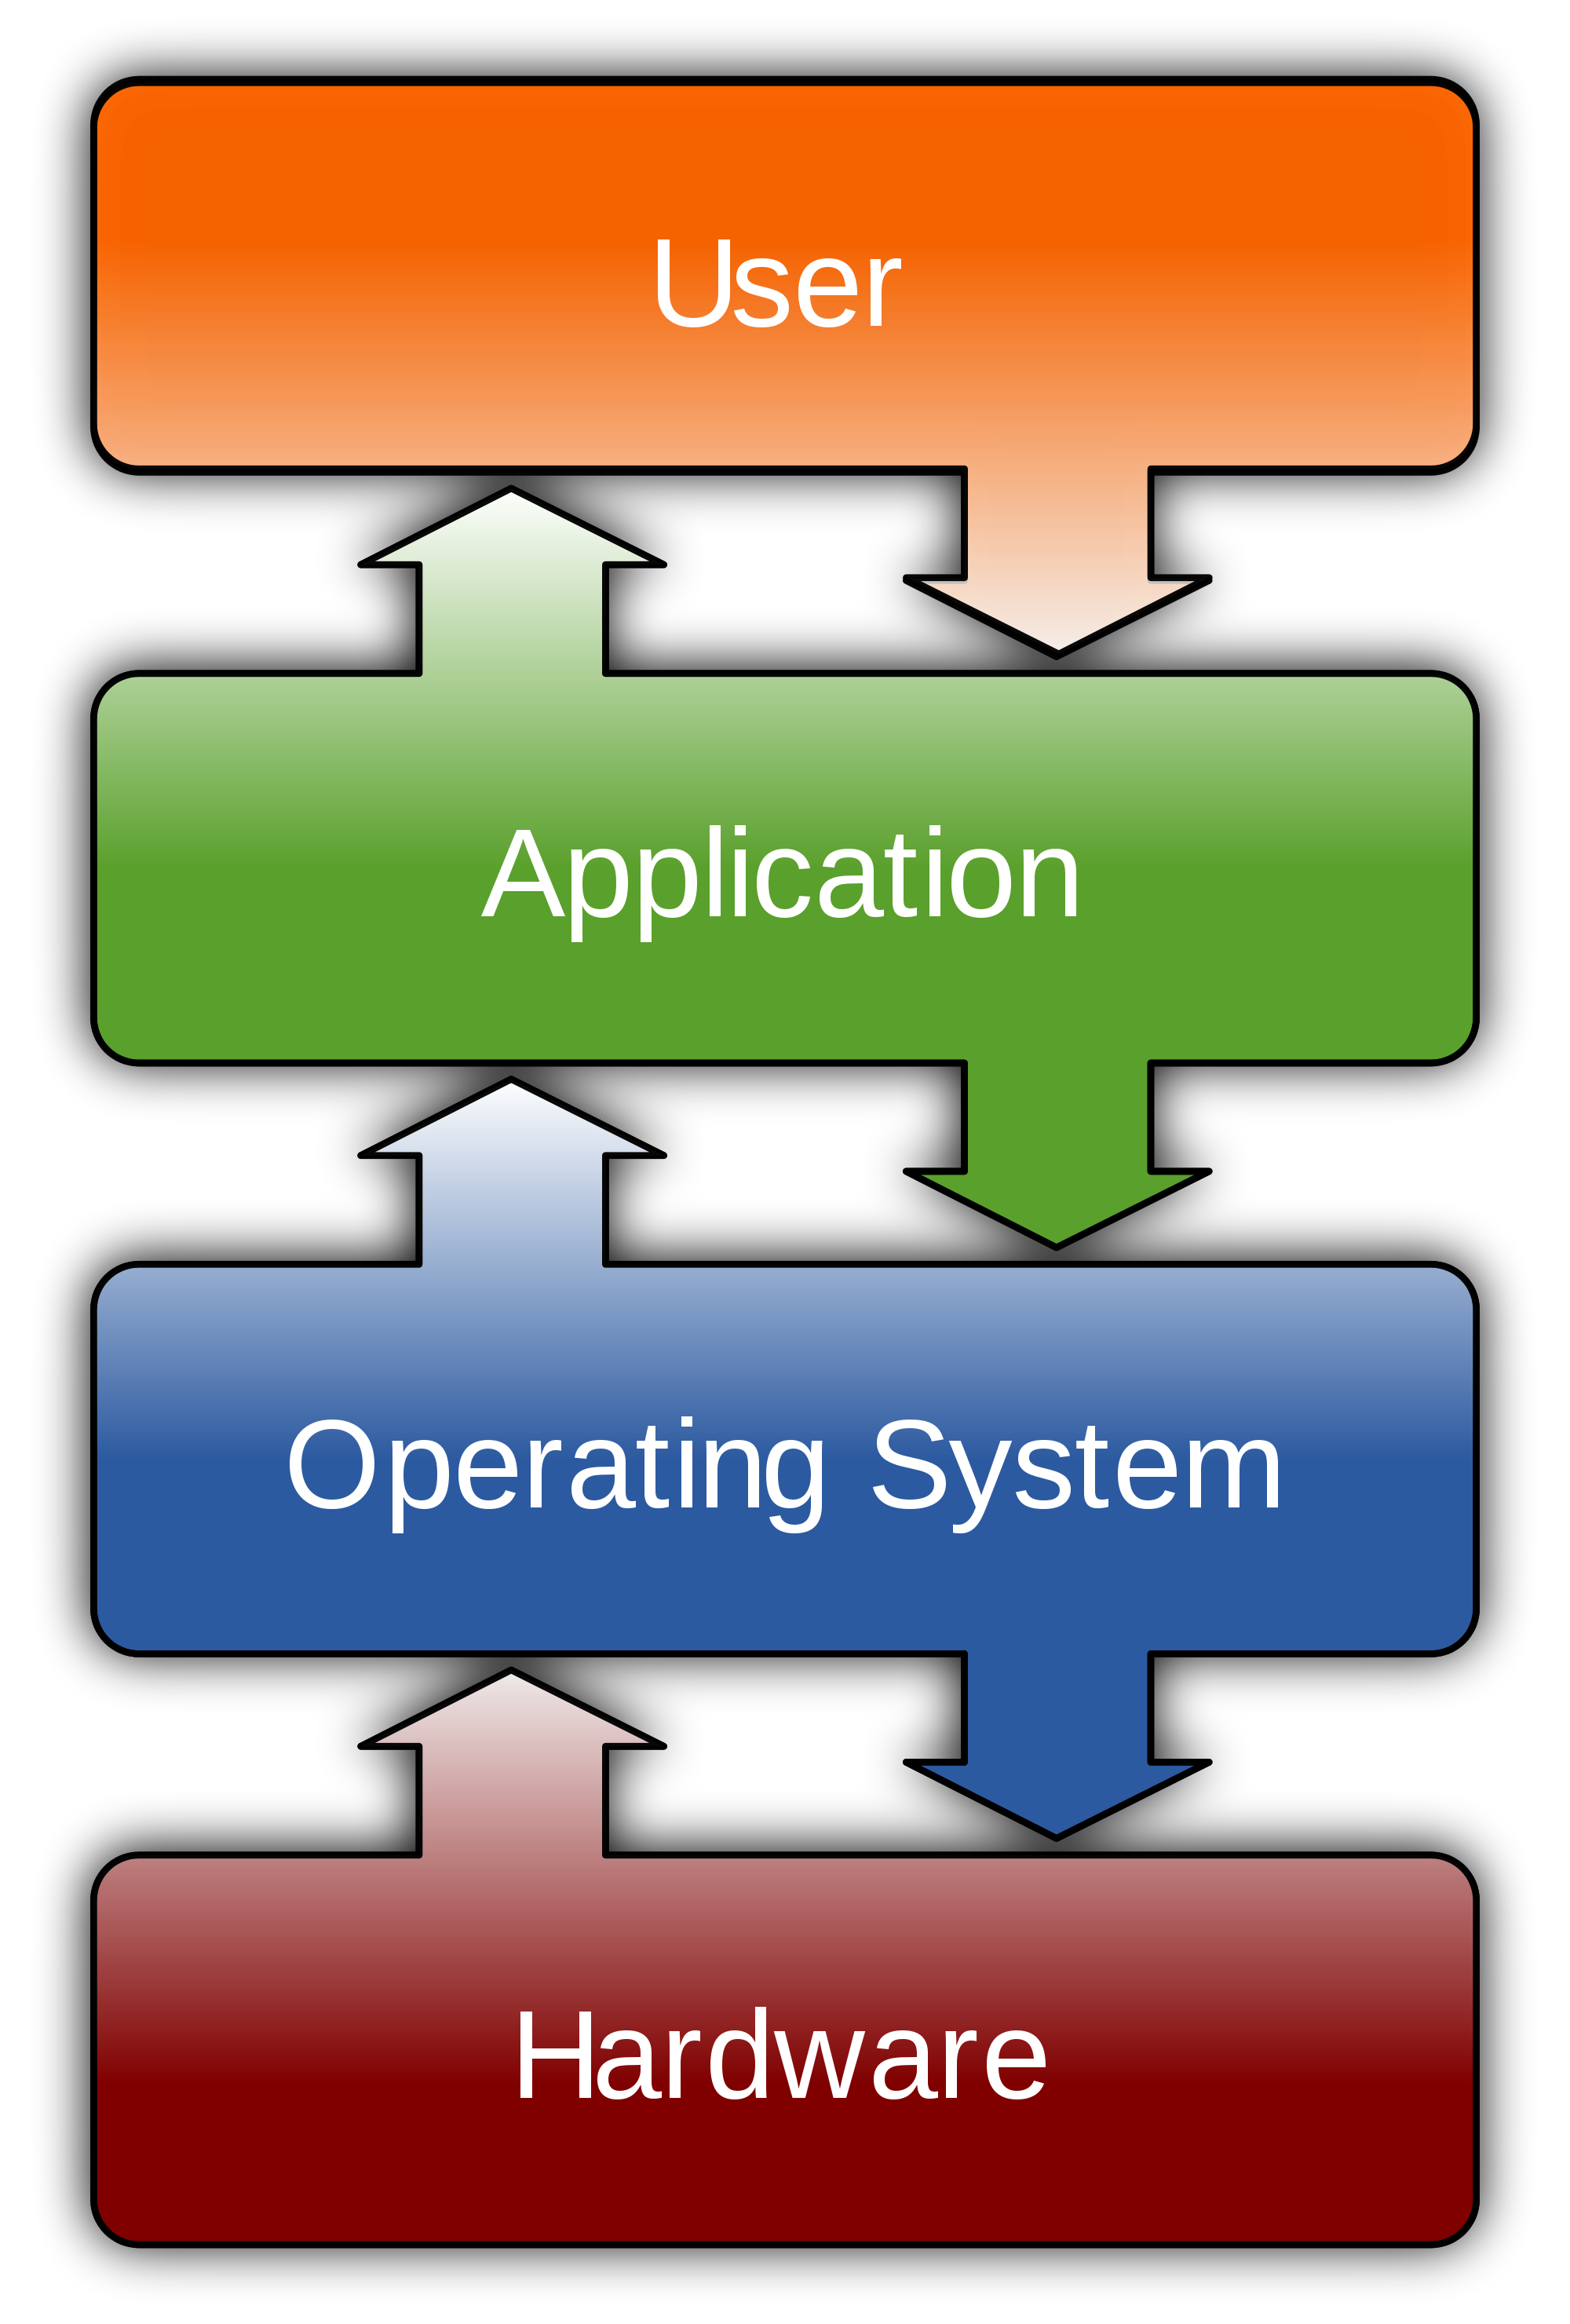
\includegraphics[scale=0.05]{images/os_diagram.png}}
    \end{figure}

	\end{columns}

\end{frame}

\subsection{Histórico}

\begin{frame}

  \begin{itemize}
  \item Criado no Bell Labs, em 1969.
  \item Seus criadores são Ken Thompson e Dennis Ritchie.
	\item Foco em modularidade, simplicidade e extensibilidade (princípio K.I.S.S.)
	\item Tudo são arquivos (literalmente, veremos melhor depois)
  \end{itemize}

	\begin{columns}
		\column{0.2\textwidth}
		\column{0.6\textwidth}

		\begin{block}{Bell Labs}
	    Laboratório onde foram criadas diversas coisas importantes para
			nós hoje:
	    \begin{itemize}
	    \item C/C++
	    \item Transistor
	    \item Laser
		  \end{itemize}
	  \end{block}

		\column{0.2\textwidth}
	\end{columns}

\end{frame}

\begin{frame}
  \begin{columns}
		\column{0.1\textwidth}
    \column{0.35\textwidth}

    \begin{block}{Dennis Ritchie}

      \begin{figure}
        \fbox{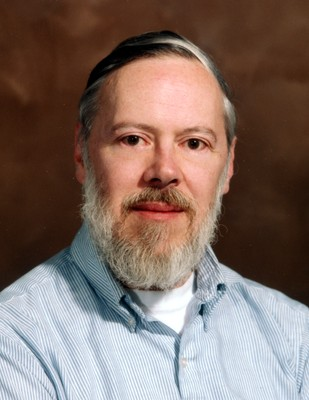
\includegraphics[scale=0.22]{images/dennis_ritchie.jpg}}
      \end{figure}

      \begin{itemize}
      \item B
      \item C
      \item MULTICS
      \end{itemize}

    \end{block}

		\column{0.1\textwidth}
    \column{0.35\textwidth}

    \begin{block}{Ken Thompson}

      \begin{figure}
        \fbox{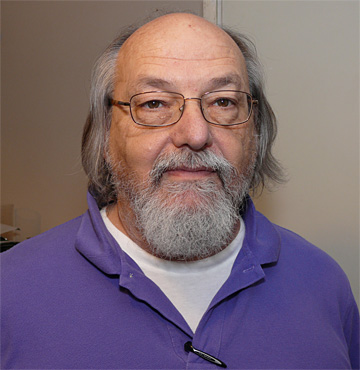
\includegraphics[scale=0.17]{images/ken_thompson.jpg}}
      \end{figure}

      \begin{itemize}
      \item B
      \item UTF-8
      \item Go
      \end{itemize}

    \end{block}

		\column{0.1\textwidth}
  \end{columns}
\end{frame}

\begin{frame}

  Hoje, ``Unix'' define uma família de sistemas operacionais que derivam
  do UNIX original.

  \begin{columns}

    \column{0.5\textwidth}
    
    \begin{block}{Unix}
      \begin{itemize}
      \item AIX
      \item Mac OS X
      \item HP-UX
      \item \ldots
      \end{itemize}
    \end{block}

    \column{0.5\textwidth}

    \begin{block}{Unix-like}
      \begin{itemize}
      \item FreeBSD
      \item GNU/Linux
      \item Minix
      \item \ldots
      \end{itemize}
    \end{block}

  \end{columns}

\end{frame}

\begin{frame}
  
  Atualmente, sistemas Unix e Unix-like são utilizados em:

  \begin{itemize}
  \item Servidores
  \item Supercomputadores
  \item Computação pessoal
    \begin{itemize}
    \item Desktops
    \item Smartphones
    \end{itemize}
  \end{itemize}

\end{frame}

\subsection{Sistema de arquivos}

\begin{frame}

	O UNIX (e seus derivados) usam um sistema de arquivos chamado FHS, o
	\textbf{Filesystem Hierarchical Standard}. Ele pode variar, mas geralmente
	segue o padrão:

	\begin{itemize}
		\item[\url{/}] a "raiz" do sistema, a base da árvore de arquivos
		\item[\url{/bin}] contém os programas essenciais, que não devem ser alterados
		\item[\url{/boot}] armazena o kernel e os arquivos necessários para o boot
		\item[\url{/dev}] representa os dispositivos conectados, como discos, mouse,
			monitores, etc.
		\item[\url{/etc}] possui os arquivos de configuração para os programas
		\item[\url{/home}] é onde ficam os diretórios pessoais dos usuários
			\newline
			Exemplo: o diretório do usuário \texttt{grad} fica em \url{/home/grad}
	\end{itemize}

\end{frame}

\begin{frame}

	(Essa árvore é bem grande)

	\begin{itemize}
		\item[\url{/lib}] contém as bibliotecas para os programas em \url{/bin} e
			\url{/sbin}
		\item[\url{/media}] é onde ficam os discos removíveis, como CDs e pendrives
		\item[\url{/mnt}] funciona como a \url{/media}, mas para dispositivos que
			não são temporários, como outros HDs internos
	\end{itemize}

	\begin{block}{Dispositivos montados}
		Quando um dispositivo com sistema de arquivos (HD, pendrive) é plugado, ele
		precisa ser \textbf{montado}. Montar um sistema de arquivos significa 
		"enxertar" a raiz desse sistema em algum ponto do seu sistema de arquivos
		principal, geralmente \url{/media} ou \url{/mnt}.
	\end{block}
	
\end{frame}

\begin{frame}
	
	\begin{itemize}
		\item[\url{/proc}] contém arquivos com dados sobre o sistema,	como as
			informações do processador, memória, e sobre os processos
		\item[\url{/root}] o \texttt{root}, que não se mistura com essa gentalha,
			tem sua home aqui, e não em \url{/home/root}
		\item[\url{/sbin}] é onde ficam os programas essenciais para manutenção
			do sistema, necessários apenas pelo \texttt{root}.
		\item[\url{/usr}] possui programas, bibliotecas e outras coisas mais que
			podem ser usadas pelos usuários comuns (não-\texttt{root}), é como a raiz
		\item[\url{/var}] armazena arquivos variáveis, como logs e bancos de dados,
			mas que devem ser preservados ao reiniciar
		\item[\url{/tmp}] ao contrário de \url{/var}, guarda arquivos temporários
			que podem ser excluídos a qualquer momento
	\end{itemize}

\end{frame}

\subsection{Sistema de usuários}

\begin{frame}

	Outro ponto do UNIX é seu sistema de usuários e permissões. Cada usuário faz
	parte de um ou mais grupos que podem indicar suas permissões. Veremos as
	permissões de um arquivo em breve.
	\newline
	\newline
	Cada conjunto de permissões possui três diretivas:
	\begin{itemize}
		\item[r] ou \textbf{read}, é a permissão de ler o conteúdo
		\item[w] ou \textbf{write}, é a permissão de alterar o conteúdo
		\item[x] ou \textbf{execute}, é a permissão de executar arquivos
	\end{itemize}
	Cada arquivo possui três conjuntos, para diferentes usuários:
	\begin{itemize}
		\item[u] ou \textbf{user}, é a permissão que o dono do arquivo tem
		\item[g] ou \textbf{group}, é a permissão que o grupo dono do arquivo tem
		\item[o] ou \textbf{others}, é a permissão que outros usuários que não o
			dono e não são do grupo dono possuem
	\end{itemize}

\end{frame}

\begin{frame}

	\begin{columns}

		\column{0.5\textwidth}
		{\huge Superusuário}

		O superusuário possui todas as permissões em todos os arquivos. Ele serve
		para fazer manutenção no sistema, pois um usuário comum não pode mexer nos
		arquivos essenciais.
		\newline
		\newline
		Geralmente ele é chamado de root e existem alguns comandos especiais para
		ser usado.

		\column{0.5\textwidth}

		\begin{figure}
			
\includegraphics[scale=0.3]{images/rambo.jpg}
	  \end{figure}

	\end{columns}

\end{frame}

\section{GNU/Linux}

\begin{frame}
  Linux é um sistema Unix-like, de fácil acesso, e muito adequado à
  computação pessoal (e não só!)

  \begin{figure}
    
\includegraphics[scale=0.2]{images/tux.png}
    \footnotesize{
    \\Tux, mascote do Linux
    \\Créditos: Larry Ewing
    \\http://en.wikipedia.org/wiki/File:Tux-simple.svg
    }
  \end{figure}
\end{frame}

\subsection{Histórico}

\begin{frame}
  O kernel Linux foi criado por Linus Torvalds em 1991.

  \begin{columns}
    \column{0.25\textwidth}
    \column{0.5\textwidth}

    \begin{block}{Linus Torvalds}

      \begin{figure}
        \fbox{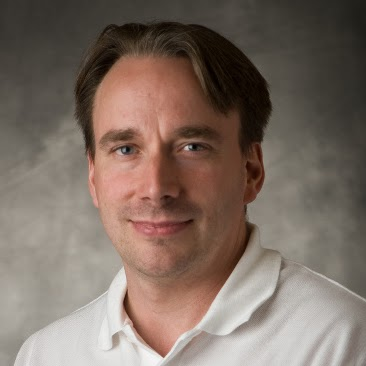
\includegraphics[scale=0.15]{images/linus_torvalds.jpg}}
      \end{figure}

      \begin{itemize}
      \item Kernel Linux
      \item Git
      \end{itemize}

    \end{block}

    \column{0.25\textwidth}
  \end{columns}

\end{frame}

\begin{frame}

  \begin{block}{Torvalds, comp.os.minix, 1991}
    \footnotesize{
      I'm doing a (free) operating system (just a hobby, won't be big and
      professional like gnu) for 386(486) AT clones.  This has been
      brewing since april, and is starting to get ready.  I'd like any
      feedback on things people like/dislike in minix, as my OS resembles
      it somewhat (same physical layout of the file-system (due to
      practical reasons) among other things).
      \newline
      \newline
      (\ldots)
      \newline
      \newline
      PS\@.  Yes - it's free of any minix code, and it has a
      multi-threaded fs. It is NOT protable (uses 386 task switching
      etc), and it probably never will support anything other than
      AT-harddisks, as that's all I have :-(. 
    }
	\end{block}

	\scriptsize{
	Disponível em: \url{https://groups.google.com/d/msg/comp.os.minix/dlNtH7RRrGA/SwRavCzVE7gJ}
	}

\end{frame}

\subsection{Kernel Linux e GNU}

\begin{frame}
  O projeto GNU, fundado por Richard Stallman, acabou adotando o kernel
  Linux como o kernel para seu sistema operacional, pois o HURD, o
  kernel que estava em desenvolvimento pela GNU estava em estágio muito
  inicial.
  
  \begin{columns}
    \column{0.25\textwidth}
    \column{0.5\textwidth}

    \begin{block}{Richard Matthew Stallman}

      \begin{figure}
        \fbox{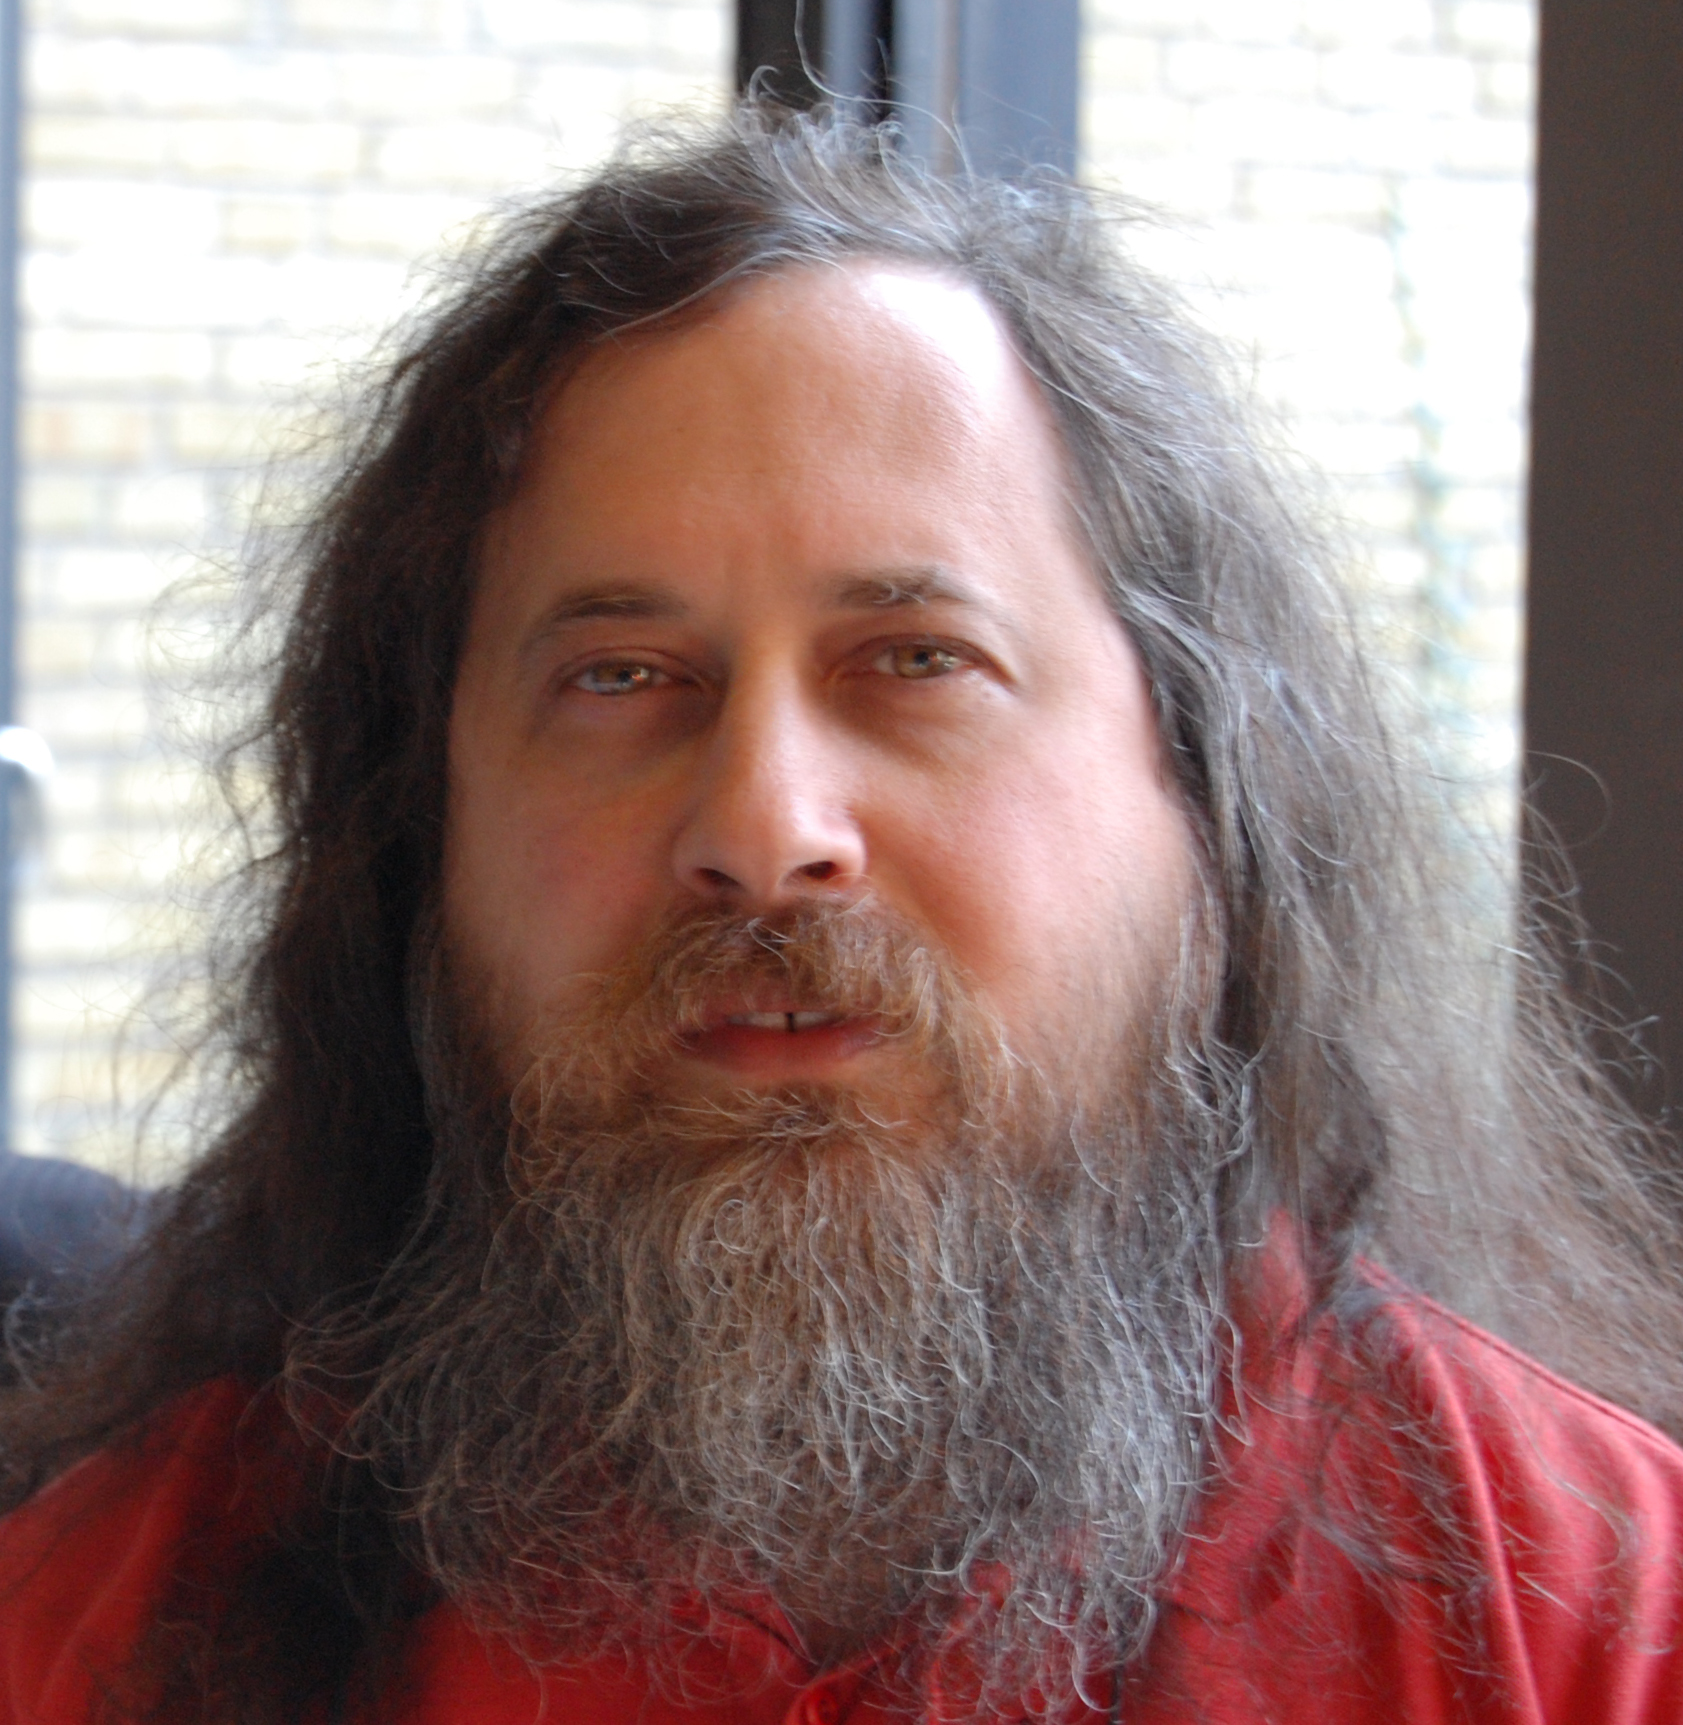
\includegraphics[scale=0.15]{images/richard_stallman.jpg}}
      \end{figure}

      \begin{itemize}
      \item GNU
      \item GNU Emacs
      \item POSIX
      \end{itemize}

    \end{block}

    \column{0.25\textwidth}
  \end{columns}
\end{frame}

\subsection{Distribuições}

\begin{frame}
  O sistema GNU/Linux possui várias distribuições. Uma distribuição
  nada mais é que um conjunto de softwares aplicativos em torno do
  kernel Linux e os utilitários GNU, de forma a atender um conjunto
  de usuários.

  \begin{columns}
    \column{0.2\textwidth}
    \column{0.6\textwidth}

    \begin{block}{Distribuições}
      \begin{itemize}
      \item Linux Mint
      \item Ubuntu
      \item Fedora
      \item Debian
      \item Arch Linux
      \item Slackware
      \item Gentoo
      \end{itemize}
    \end{block}

    \column{0.2\textwidth}
  \end{columns}

\end{frame}

\begin{frame}

  Toda distribuição é definida, basicamente, por como os programas
  disponíveis são empacotados e instalados. Na maior parte dos casos,
  isso é feito com um gerenciador de pacotes, como:

  \begin{itemize}
  \item portage
  \item pacman
  \item yum
  \item apt
  \end{itemize}

\end{frame}

\begin{frame}

	As distros geralmente se encaixam em dois tipos de atualizações (releases):
	\begin{itemize}
		\item[\textit{stable}] são distros que possuem versões bem definidas
			e, entre uma versão e outra, são feitas apenas atualizações de segurança
			e correções de bugs.
			\newline
			Exemplos: Ubuntu, Debian, Linux Mint
		\item[\textit{rolling}] são distros sem versões definidas, ou seja
			a atualização sempre vai trazer a versão mais recente dos aplicativos.
			\newline
			Exemplos: Arch Linux, Slackware, Gentoo
	\end{itemize}

	Uma distro em particular não se encaixa em nenhum: o Fedora possui versões,
	mas é atualizado como um \textit{rolling release}.

\end{frame}

\section{Hands-on}
\subsection{O terminal}

\begin{frame}

	Por que usar o terminal?

	\begin{itemize}
	\item Interface gráfica é limitada
	\item Terminal é mais rápido e simples
	\item Basta saber digitar e ler o manual
	\end{itemize}

\end{frame}

\begin{frame}

	O que é o terminal?

	\begin{itemize}
		\item Interpretador de ``comandos''
		\item Comandos geralmente são programas
		\item Programas aceitam argumentos e opções
	\end{itemize}

\end{frame}

\subsection{Resposta para a vida, o universo e tudo mais}

\begin{frame}

	\large{O comando \textbf{mais importante} de todos é o \texttt{man}. Com ele, você
	pode ler o manual de instruções de qualquer outro - até o dele mesmo.}
	\newline
	\newline
	Sempre use este comando quando estiver em dúvida!

\end{frame}

\subsection{Manipulando diretórios e arquivos}

\begin{frame}

	Para mudar de diretório, use \texttt{cd <diretório>}.
	\newline
	\newline
	Para saber onde você está, use \texttt{pwd}.
	\newline
	\newline
	Para listar o conteúdo de um diretório, use \texttt{ls}.

	\begin{block}{Flags do \texttt{ls}}
		O comando \texttt{ls} aceita as \textit{flags} \texttt{-a} e \texttt{-l},
		além de várias outras. Tente usá-las e combiná-las para entender o que
		elas fazem!
	\end{block}

\end{frame}

\begin{frame}
	
	Se você precisar de um novo diretório, use \texttt{mkdir <diretório>}.
	\newline
	\newline
	Você pode usar \texttt{touch <arquivo>} ou \texttt{> <arquivo>} para criar um arquivo.
	\newline
	\newline
	Para remover um arquivo, use \texttt{rm}. Um diretório pode ser removido usando a \textit{flag} \texttt{-r}, que significa \textbf{recursive}.

	\begin{alertblock}{Cuidado com o \texttt{rm}}
		Um arquivo ou	diretório removido com \texttt{rm} não é enviado para uma
		lixeira, ele é perdido para sempre! Sempre tome	cuidado quando for remover
		algo para não perder nada importante.
	\end{alertblock}

\end{frame}

\begin{frame}

	Além de criar e remover arquivos, também podemos copiar e mover eles por aí.
	\newline
	\newline
	Podemos copiar um arquivo usando \texttt{cp <origem> <destino>}. O destino
	pode ser um diretório ou arquivo.
	\newline
	\newline
	Para mover um arquivo, usamos \texttt{mv <origem> <destino>}. Também serve
	para renomear um arquivo.

\end{frame}

\begin{frame}

	Existem alguns caminhos especiais para facilitar:

	\begin{itemize}
		\item[.] significa o diretório atual
		\item[..] significa o diretório "pai" ou superior
		\item[-] é o diretório visitado anteriormente
		\item[\url{~}] é o diretório pessoal do usuário atual
		\item[\url{~user}] é o diretório pessoal de \texttt{user}
	\end{itemize}

\end{frame}

\begin{frame}

	Também existem \textit{wildcards} para manipular arquivos e diretórios:

	\begin{itemize}
		\item[*] casa com qualquer ocorrência
			\newline
			Exemplo: \texttt{rm \url{~/Pictures/*.jpg}} remove todos os arquivos cujos nomes
			terminam em \texttt{.jpg} no diretório \texttt{\url{~/Pictures}}.
		\item[?] casa com qualquer caractere, mas apenas um
			\newline
			Exemplo: \texttt{ls arq?} pode encontrar \texttt{arq1}, \texttt{arqc}, etc.
		\item[{[ ]}] casa qualquer ocorrência no intervalo
			\newline
			Exemplo: \texttt{rm arq[1-3]} remove os arquivos \texttt{arq1},
			\texttt{arq2} e \texttt{arq3} apenas.
		\item[\{\}] casa com as ocorrências definidas em uma lista
			\newline
			Exemplo: \texttt{mkdir dir\{,test,\_pet\}} cria os diretórios \texttt{dir},
			\texttt{dirtext} e \texttt{dir\_pet}.
	\end{itemize}

\end{frame}

\subsection{Lendo e alterando arquivos}

\begin{frame}

	Existem alguns comandos que podemos usar para ver e alterar o conteúdo de um arquivo:

	\begin{itemize}
		\item[\texttt{cat}] é utilizado para concatenar arquivos e exibir.
			\newline
			Exemplo: \texttt{cat arq1 arq2} mostra o conteúdo dos arquivos arq1 e arq2.
			\newline
			\begin{block}{Curiosidade sobre o \texttt{cat}}
				Se colocarmos apenas um arquivo, ele vai mostrar o que esse arquivo tem.
				E, como tudo são arquivos, também podemos ler, por exemplo, a entrada do
				mouse: tente usar \texttt{cat /dev/input/mice} quando for \texttt{root}.
			\end{block}
	\end{itemize}

\end{frame}

\begin{frame}

	\begin{itemize}
		\item[\texttt{head}] mostra o início de um arquivo. Com a \textit{flag}
			\texttt{-n x}, mostra as \texttt{x} primeiras linhas, e \texttt{-n -x}
			mostra todas menos as \texttt{x} últimas.
		\item[\texttt{tail}] mostra o final de um arquivo, funciona igual ao
			\texttt{head}.
		\item[\texttt{less}] é usado para ler o conteúdo de um arquivo linha por
			linha, permite subir e descer	pelas linhas de um arquivo.
		\item[\texttt{echo}] é usado para escrever algo, podemos usar \texttt{>}
			para direcionar para um arquivo.
			\newline
			Exemplo: \texttt{echo hello > arq.txt} escreverá "hello" em \texttt{arq.txt}.
		\item[editores] Existem diversas opções: o \texttt{nano}, mais simples, e
			o \texttt{vi}, mais completo, são os mais	populares.
	\end{itemize}
\end{frame}

\subsection{Usuários e grupos}

\begin{frame}

	Podemos usar \texttt{su <user>} para logar como \texttt{user} (ou deixar em
	branco para \texttt{root}). É necessário informar a senha, se houver.
	\newline
	\newline
	Semelhante ao \texttt{su}, é possível executar um comando como outro usuário
	usando \texttt{sudo -u <user> <comando>}. Da mesma forma, é necessário saber
	a senha, e o usuário padrão é o \texttt{root}.
	\newline
	\newline
	Você pode mudar sua senha usando \texttt{passwd}. O usuário \texttt{root}
	pode mudar a senha de qualquer um com \texttt{passwd <user>}.

\end{frame}

\begin{frame}

	O comando \texttt{users} mostra os usuários logados atualmente. O comando
	\texttt{who} faz isso de uma forma mais detalhada.
	\newline
	\newline
	Para saber que usuário você está usando, existe o comando \texttt{whoami}
	\newline
	\newline
	Os grupos de um usuário podem ser conferidos com o comando
	\texttt{groups <user>}, sendo que o padrão é o usuário atual.

\end{frame}

\subsection{Permissões}

\begin{frame}

	Podemos alterar o usuário e o grupo donos de um arquivo com \texttt{chown} e
	\texttt{chgrp}:
	\begin{itemize}
		\item Alteramos o usuário com \texttt{chown <user> <arquivo>}
		\item Alteramos o grupo com \texttt{chgrp <group> <arquivo>}
		\item Alternativamente, \texttt{chown <user>:<group> <arquivo>}
	\end{itemize}
	Exemplo:
	\begin{itemize}
		\item \texttt{chown pet:ufsc unix.pdf teste.txt} muda o usuário e o grupo
		\textbf{unix.pdf} e \textbf{teste.txt} para \textbf{pet} e \textbf{ufsc}
	\end{itemize}

\end{frame}

\begin{frame}

	Já os grupos de permissões podem ser alterados com \texttt{chmod}. Podemos
	adicionar e remover permissões usando os sinais \texttt{+} e \texttt{-}.
	\newline
	Exemplos:
	\begin{itemize}
		\item \texttt{chmod g+rx unix.pdf} adiciona permissão de leitura e execução
			aos membros do grupo dono de \textbf{unix.pdf}
		\item \texttt{chmod a-rwx foo.bar} remove todas as permissões de todos os
			usuários para \textbf{foo.bar} (\texttt{a} significa \textbf{all}, todos)
	\end{itemize}

\end{frame}

\section{}

\begin{frame}
	\Huge{Dúvidas?}

	
\includegraphics{images/tux.png}
\end{frame}

\begin{frame}
  This work is licensed under the Creative Commons Attribution-ShareAlike 4.0 International License. To view a copy of this license, visit \url{http://creativecommons.org/licenses/by-sa/4.0/}.
\end{frame}

\end{document}
